\documentclass[a4paper,12pt]{extarticle}
\usepackage{geometry}
\usepackage[T1]{fontenc}
\usepackage[utf8]{inputenc}
\usepackage[english,russian]{babel}
\usepackage{amsmath}
\usepackage{amsthm}
\usepackage{amssymb}
\usepackage{fancyhdr}
\usepackage{setspace}
\usepackage{graphicx}
\usepackage{colortbl}
\usepackage{tikz}
\usepackage{pgf}
\usepackage{subcaption}
\usepackage{listings}
\usepackage{indentfirst}
\usepackage[
backend=biber,
style=numeric,
maxbibnames=99
]{biblatex}
\addbibresource{refs.bib}
% Bibliography list labels: "1." instead of "[1]" (numeric.bbx uses labelnumberwidth + mkbibbrackets)
\DeclareFieldFormat{labelnumberwidth}{#1.}
\usepackage[colorlinks,citecolor=blue,linkcolor=blue,bookmarks=false,hypertexnames=true, urlcolor=blue]{hyperref} 
\usepackage{indentfirst}
\usepackage{mathtools}
\usepackage{booktabs}
\usepackage[flushleft]{threeparttable}
\usepackage{tablefootnote}

\usepackage{chngcntr} % нумерация графиков и таблиц по секциям
\counterwithin{table}{section}
\counterwithin{figure}{section}

\graphicspath{{graphics/}}%путь к рисункам

\geometry{left=2.5cm}% левое поле
\geometry{right=1.0cm}% правое поле
\geometry{top=2.0cm}% верхнее поле
\geometry{bottom=2.0cm}% нижнее поле
\setlength{\parindent}{1.25cm}
\renewcommand{\baselinestretch}{1.5} % междустрочный интервал


\newcommand{\bibref}[3]{\hyperlink{#1}{#2 (#3)}} % biblabel, authors, year
\addto\captionsrussian{\def\refname{Список литературы (или источников)}} 

\renewcommand{\theenumi}{\arabic{enumi}}% Меняем везде перечисления на цифра.цифра
\renewcommand{\labelenumi}{\arabic{enumi}}% Меняем везде перечисления на цифра.цифра
\renewcommand{\theenumii}{.\arabic{enumii}}% Меняем везде перечисления на цифра.цифра
\renewcommand{\labelenumii}{\arabic{enumi}.\arabic{enumii}.}% Меняем везде перечисления на цифра.цифра
\renewcommand{\theenumiii}{.\arabic{enumiii}}% Меняем везде перечисления на цифра.цифра
\renewcommand{\labelenumiii}{\arabic{enumi}.\arabic{enumii}.\arabic{enumiii}.}% Меняем везде перечисления на цифра.цифра

\begin{document}
\begin{titlepage}
\newpage
% Single spacing on title page: document uses 1.5 linespread, which overflows with two students.
{\setstretch{1.0}\selectfont
\begin{center}
{\bfseries
\MakeUppercase{Федеральное государственное автономное образовательное}\\
\MakeUppercase{учреждение высшего образования}\\
\MakeUppercase{«Национальный исследовательский университет}\\
\MakeUppercase{«Высшая школа экономики»}\\
\MakeUppercase{Факультет компьютерных наук}
}
\end{center}

\vspace{3em}

\begin{center}
\underline{Ахундов Алексей Назимович, Жарковский Дмитрий Андреевич}
\end{center}

\vspace{2em}

\begin{center}
МАГИСТЕРСКАЯ ДИССЕРТАЦИЯ\\[0.5em]
{\bf \underline{Генерация персонализированных учебных конспектов по предметам ЕГЭ}}\\[0.3em]
{\bf \underline{на основе языковых моделей и пользовательской аналитики}}
{\bf \underline{Generation of Personalized Educational Notes for Unified State Exam Subjects}}
{\bf \underline{Based on Language Models and User Analytics}}
\end{center}

\vspace{2em}

\begin{center}
{\setstretch{1.2}
по направлению подготовки \underline{01.04.02 Прикладная математика и информатика}\\
образовательная программа «Искусственный интеллект»
}
\end{center}

\vfill

\noindent
\begin{minipage}[t]{0.45\textwidth}
Студент\\[1em]
\rule{5cm}{0.4pt}\\
А.Н. Ахундов\\[1em]
Студент\\[1em]
\rule{5cm}{0.4pt}\\
Д.А. Жарковский
\end{minipage}%

\hfill
\begin{minipage}[t]{0.5\textwidth}
\raggedleft
Научный руководитель\\
Кандидат физико-математических наук\\[1em]
\rule{5cm}{0.4pt}\\
Е.О. Кантонистова\\[1.25em]

Соруководитель\\
Преподаватель\\[1em]
\rule{5cm}{0.4pt}\\
П.И. Ахтямов
\end{minipage}

\vspace{2em}

\begin{center}
Москва 2026
\end{center}

}
\end{titlepage}
% это титульный лист - выберите подходящий вам из имеющихся в проекте вариантов (kr - курсовая работа у 3 курса, vkr - выпускная квалификационная работа у 4 курса)
\newpage
\setcounter{page}{2}

{
	\hypersetup{linkcolor=black}
	\tableofcontents
}

\newpage

\newpage
\section*{Аннотация}   % this is how to use russian
Здесь будет аннотация на русском языке

\addcontentsline{toc}{section}{Аннотация}

\section*{Ключевые слова}
Глубинное обучение, разреживание моделей, рекуррентные нейронные сети
\pagebreak


\section*{Abstract}   % this is how to use english
Your abstract in English.

\addcontentsline{toc}{section}{Abstract}

\section*{Keywords}
Deep learning, model pruning, recurrent neural networks
\pagebreak


\section*{Введение}
Текст введения.
\addcontentsline{toc}{section}{Введение}
\pagebreak


\section{
    Глава 1. Проблематика персонализированного онлайн-обучения 
    и постановка задачи генерации учебных конспектов
}

\subsection{Цифровизация подготовки к ЕГЭ и особенности рынка онлайн-обучения}

Подготовка к ЕГЭ за последние годы стала одной из наиболее заметных областей цифрового образования. 
На рынке одновременно присутствуют крупные образовательные платформы и специализированные онлайн-школы, 
предлагающие курсы, тренажеры, видеоразборы и консультации по предметам экзамена. 
Это подтверждается как распространенностью профильных сервисов, так и разнообразием их продуктовых моделей: 
отдельные предметные курсы и тренажеры представлены, например, 
у Яндекса, ЕГЭLand, Умскул и MAXIMUM~\cite{maximum2026ege,egeland2026,umschool2026,yandex2026ege_math}. 
Для пользователя такой рынок создает широкий выбор форматов, однако одновременно усиливает конкуренцию 
по качеству контента, степени персонализации и скорости адаптации материалов под конкретные образовательные цели.

Современные исследования онлайн-образования показывают, что эффективность цифрового обучения определяется не только 
наличием учебных материалов, но и качеством структуры курса, уровнем интерактивности, развитием саморегуляции 
обучающегося, цифровой грамотностью и институциональной поддержкой~\cite{vandorresteijn2025online}. 
Иными словами, простой перенос теории и задач в веб-интерфейс еще не делает обучение по-настоящему эффективным. 
Особенно остро это проявляется в экзаменационной подготовке, где учащемуся нужен не просто доступ к контенту, 
а своевременное объяснение именно тех тем, которые вызывают устойчивые ошибки.

Для подготовки к ЕГЭ эта проблема имеет особую специфику. Во-первых, содержание обучения жестко ограничено 
кодификатором и спецификацией экзамена, поэтому образовательный сервис должен обеспечивать релевантность и 
нормативную корректность материалов. Во-вторых, темп усвоения тем у разных учеников заметно различается: один 
обучающийся испытывает трудности с базовыми определениями, другой --- с типовыми преобразованиями, третий --- 
с переносом знаний на задания повышенной сложности. В-третьих, массовые онлайн-курсы обычно строятся вокруг 
усредненной траектории: ученик получает одинаковую теорию, общий набор практики и ограниченную адаптацию, 
выраженную чаще всего в рекомендации следующего урока или задания.

Таким образом, на рынке онлайн-подготовки сформировалось противоречие. С одной стороны, цифровые платформы 
обеспечивают масштабируемость, доступность и богатую учебную аналитику. С другой стороны, они по-прежнему 
редко предоставляют персонализированный теоретический материал в форме связного учебного конспекта, отражающего 
историю ошибок, текущий уровень подготовки и учебные цели конкретного ученика. Именно это противоречие и 
определяет актуальность разработки специализированного сервиса для платформы ЕГЭПрорыв~\cite{exambreakout2026}.

\subsection{Научно-прикладные подходы к персонализации обучения}

В научной литературе персонализированное обучение понимается как организация учебного процесса, при которой 
содержание, темп, форма представления материала и обратная связь адаптируются под особенности конкретного 
обучающегося~\cite{khor2024la}. Такой подход противопоставляется модели ``one-size-fits-all'', в которой один 
и тот же учебный материал предъявляется всей аудитории без учета различий в исходной подготовке, стиле усвоения 
и динамике прогресса.

Методологической основой персонализации выступают learning analytics и educational data mining. По определению 
R. Baker, образовательный data mining ориентирован на извлечение закономерностей из учебных данных для понимания 
и оптимизации обучения~\cite{baker2010edm}. В более позднем обзоре C. Romero и S. Ventura подчеркивается, 
что learning analytics и educational data mining сегодня образуют единую исследовательскую область, 
в которой анализ цифровых следов обучающегося используется для прогнозирования результатов, выявления трудностей 
и поддержки педагогических решений~\cite{romero2020edm}. Систематический обзор E. T. Khor и M. K показывает, 
что learning analytics способствует персонализации как минимум по пяти направлениям: сбор данных о прогрессе, 
классификация учащихся, построение циклов обратной связи, прогнозирование результатов и предоставление 
преподавателю или системе интерпретируемых рекомендаций в реальном времени~\cite{khor2024la}.

Отдельное место в персонализации занимает моделирование знаний обучающегося. Классической работой в 
этой области считается статья A. Corbett и J. Anderson, где была предложена модель knowledge 
tracing для оценки вероятности усвоения навыка по последовательности ответов ученика~\cite{corbett1994kt}. 
Дальнейшее развитие направление получило в работе C. Piech и соавторов о deep knowledge tracing, 
где динамика овладения знаниями моделируется с помощью нейросетевых методов~\cite{piech2015dkt}. 
Современный обзор G. Abdelrahman и соавторов показывает, что learner modeling и knowledge tracing остаются 
центральными инструментами адаптивных обучающих систем, особенно в задачах прогнозирования ошибок, 
выбора индивидуальной траектории и адресной поддержки~\cite{abdelrahman2023ktsurvey}.

Новый этап развития персонализации связан с большими языковыми моделями. Работы по BERT, GPT и LLaMA показали, 
что крупные трансформерные модели способны решать широкий круг задач понимания и генерации текста, 
включая объяснение понятий, переформулирование материала и адаптацию стиля 
изложения~\cite{devlin2019bert,brown2020gpt3,touvron2023llama}. 
Для образования это особенно важно, поскольку учебный контент является прежде всего текстовым знанием, 
которое должно быть представлено в понятной, логичной и методически корректной форме.

При этом использование LLM в образовании нельзя сводить к обычному чат-интерфейсу. Обзор E. Kasneci и 
соавторов показывает, что большие языковые модели открывают значительные возможности для тьюторской поддержки, 
генерации объяснений и автоматизации обратной связи, однако одновременно создают риски недостоверности, 
избыточной уверенности модели и педагогически неудачных подсказок~\cite{kasneci2023chatgpt}. 
Систематический обзор L. Yan и соавторов дополняет этот вывод практическими и этическими ограничениями: 
зависимость обучающихся от подсказок ИИ, непрозрачность алгоритмических решений, проблемы приватности и 
справедливости, а также сложность надежной оценки качества сгенерированного материала~\cite{yan2024challenges}. 
Более свежий систематический обзор Y. Shi и соавторов подтверждает, что LLM уже активно применяются 
в интеллектуальных обучающих системах, но их положительный эффект оказывается неоднородным и сильно зависит от 
сценария внедрения, глубины педагогической интеграции и наличия внешнего контроля~\cite{shi2025llmedu}.

Для повышения надежности генерации используются retrieval-augmented generation и агентные архитектуры. 
Подход RAG предполагает дополнение генерации внешним контекстом из базы знаний, что снижает вероятность 
галлюцинаций и делает ответы более привязанными к предметной области~\cite{lewis2020rag,gao2024ragsurvey}. 
В образовательном контексте, как показывает обзор Y. Ding и соавторов, RAG особенно полезен тогда, 
когда необходимо связать генерацию с учебной программой, проверенными материалами и профилем 
ученика~\cite{ding2025ragedu}. Агентные системы, в свою очередь, позволяют разнести функции анализа, 
планирования, генерации и проверки между несколькими взаимосвязанными компонентами, а библиотека LangGraph 
используется именно для построения управляемых stateful-пайплайнов такого типа~\cite{langchain2024}. 
Для образовательных решений это означает возможность перейти от одиночного ответа модели к воспроизводимому 
конвейеру подготовки учебного материала.

\subsection{Критический анализ существующих решений и исследований}

Существующие решения в предметной области можно условно разделить на три класса: массовые онлайн-курсы и 
платформы подготовки к экзаменам, интеллектуальные тьюторские системы на основе аналитики обучения и современные 
LLM-ориентированные AI-ассистенты.

Первый класс представлен образовательными платформами, ориентированными на массовый сегмент подготовки 
к ЕГЭ~\cite{yandex2026ege_math,egeland2026,umschool2026,maximum2026ege}. Их сильными сторонами являются 
масштабируемость, насыщенная медиатека, наличие тренажеров и готовых учебных траекторий. Однако такие решения 
обычно адаптируют обучение на уровне выбора курса, темы или набора задач, а не на уровне глубокой реконфигурации 
самого объяснения учебного материала. В результате теория остается относительно универсальной, а ученик с 
повторяющимися ошибками нередко вынужден самостоятельно собирать для себя ``личный конспект'' из видео, заметок, 
чатов и разрозненных комментариев преподавателя.

Второй класс включает системы, основанные на learner modeling, knowledge tracing и учебной 
аналитике~\cite{corbett1994kt,piech2015dkt,abdelrahman2023ktsurvey,khor2024la}. Эти подходы хорошо решают задачи 
диагностики: они позволяют определить вероятность усвоения навыка, выявить ``узкие места'' и спрогнозировать риск 
неуспешности. Их принципиальное ограничение состоит в том, что они отвечают на вопрос 
``что именно ученик знает плохо'', но не решают в полной мере вопрос 
``как именно представить этому ученику новый материал''. 
Иными словами, аналитика эффективно обнаруживает дефицит, но сама по себе не создает качественное 
персонализированное объяснение.

Третий класс --- это LLM-ориентированные образовательные ассистенты и AI-тьюторы. На прикладном уровне к 
наиболее заметным примерам относятся Khanmigo и Q-Chat~\cite{khanmigo2025,qchat2025}. На научном уровне активно 
развиваются работы по генерации персонализированной обратной связи и рекомендаций с 
помощью LLM~\cite{pankiewicz2025feedback,wang2025tutorllm}. Достоинство этих решений заключается в 
естественности взаимодействия и способности адаптировать объяснение к запросу пользователя. Тем не менее 
большинство таких систем по-прежнему работает в реактивном диалоговом режиме: они хорошо отвечают на вопрос, 
но хуже формируют целостный учебный текст, который последовательно раскрывает тему, объясняет проблемные места, 
удерживает необходимую глубину и при этом не выходит за рамки предметного стандарта.

Критический анализ литературы позволяет выделить несколько нерешенных проблем.

\begin{enumerate}
    \item \textbf{Недостаточная персонализация теоретического материала.} Обзоры по learning analytics показывают, 
	что данные о прогрессе ученика могут использоваться для классификации, прогнозирования и формирования обратной 
	связи~\cite{khor2024la}. Однако в массовых онлайн-курсах эти данные редко преобразуются в автоматически 
	создаваемый учебный конспект, который учитывает именно слабые темы конкретного обучающегося.
    \item \textbf{Фрагментарность чатового формата.} LLM-тьюторы удобны для диалога, но учебный процесс при 
	подготовке к ЕГЭ требует не только ответов на локальные вопросы, но и системного объяснения темы в логически 
	связанной форме. По этой причине чат-ориентированный интерфейс не всегда закрывает потребность в 
	структурированном повторении материала~\cite{kasneci2023chatgpt,shi2025llmedu}.
    \item \textbf{Риски недостоверности и педагогической несогласованности.} Без внешних ограничений LLM могут 
	генерировать правдоподобный, но методически неудачный или частично некорректный текст. Для образования это 
	критично, поскольку ошибка в объяснении быстро тиражируется и закрепляется у 
	обучающегося~\cite{yan2024challenges,ding2025ragedu}.
    \item \textbf{Недостаточная прозрачность и доверие к персонализирующим алгоритмам.} Human-centered обзоры по 
	LA/AI in education показывают, что успешное внедрение образовательного ИИ требует учета вопросов контроля 
	человека, надежности, безопасности и доверия пользователей, а также внятного обоснования того, почему система 
	предлагает именно такой материал~\cite{alfredo2024human}.
\end{enumerate}

Следовательно, перспективным направлением является объединение трех линий развития: учебной аналитики как источника
 персонализирующего сигнала, LLM как механизма генерации содержательного текста и агентной оркестрации как способа 
 сделать генерацию многошаговой, контролируемой и воспроизводимой. Именно такая интеграция позволяет перейти от 
 универсального цифрового курса и реактивного чат-бота к сервису, создающему персонализированный учебный конспект 
 как самостоятельный образовательный артефакт.

\subsection{Постановка задачи ВКР и методы ее решения}

Объектом исследования в данной работе является процесс персонализированной подготовки обучающихся к ЕГЭ в цифровой 
образовательной среде. Предмет исследования --- методы и программные средства генерации учебных конспектов, 
адаптированных к индивидуальным особенностям обучающегося на основе данных пользовательской аналитики и возможностей 
больших языковых моделей.

Целью выпускной квалификационной работы является разработка сервиса для веб-ресурса ЕГЭПрорыв~\cite{exambreakout2026}, 
который автоматически формирует персонализированные учебные конспекты по предметам ЕГЭ с учетом текущего уровня 
подготовки ученика, его истории ошибок и динамики освоения тем.

Исходя из проведенного обзора, для достижения поставленной цели необходимо решить следующие задачи:

\begin{enumerate}
    \item проанализировать существующие подходы к персонализации обучения, генерации учебных материалов и 
	использованию LLM в образовательных сервисах;
    \item определить состав пользовательской аналитики, достаточной для адаптации содержания конспекта: 
	изученные темы, типовые ошибки, показатели успеваемости, частоту повторных затруднений и уровень освоения навыков;
    \item разработать структуру конспекта, в которой глубина объяснения, выбор примеров, акценты на типичных 
	ошибках и объем повторения зависят от профиля конкретного ученика;
    \item спроектировать агентную систему генерации на базе LangChain и LangGraph, разделяющую этапы анализа 
	входных данных, планирования структуры конспекта, генерации текста и внутренней проверки 
	результата~\cite{langchain2024};
    \item обеспечить управляемость генерации за счет внешних ограничений предметной области, в том числе опоры 
	на учебные материалы, специфику экзамена и контролируемую подачу контекста модели~\cite{lewis2020rag,ding2025ragedu};
    \item определить критерии качества получаемого конспекта: релевантность теме, уровень персонализации, 
	логичность структуры, читаемость, фактологическая корректность и пригодность для практического использования 
	в учебном процессе.
\end{enumerate}

Разрабатываемый сервис должен принимать на вход тему или раздел предмета ЕГЭ, профиль обучающегося и агрегированные 
данные о его взаимодействии с платформой. В качестве входной аналитики могут выступать результаты решения заданий, 
сведения о частоте ошибок по конкретным типам задач, история прохождения тем, показатели повторного обращения 
к материалу и иные характеристики, отражающие реальное состояние освоения курса. Выходом системы должен быть 
связный конспект, который содержит краткое введение в тему, адаптированное объяснение ключевых понятий, 
разбор типичных ошибок, примеры решения и рекомендации по дальнейшему изучению.

Метод решения поставленной задачи основан на сочетании трех компонентов. Первый компонент --- learner modeling и 
learning analytics, необходимые для построения информативного профиля ученика и выявления содержательных 
пробелов~\cite{khor2024la,abdelrahman2023ktsurvey}. Второй компонент --- большая языковая модель, обеспечивающая 
генерацию связного педагогически ориентированного текста~\cite{kasneci2023chatgpt,shi2025llmedu}. 
Третий компонент --- агентная orchestration-логика на базе LangChain/LangGraph, обеспечивающая разделение ролей 
внутри конвейера генерации, сохранение состояния и управляемое прохождение этапов анализа, планирования и 
синтеза ответа~\cite{langchain2024}.

С практической точки зрения разрабатываемая система должна удовлетворять следующим ограничениям:

\begin{enumerate}
    \item \textbf{предметная корректность} --- содержание конспекта не должно выходить за рамки школьной программы 
	и формата ЕГЭ;
    \item \textbf{персонализированность} --- объяснение должно учитывать реальные пробелы ученика, а не 
	ограничиваться формальным упоминанием его уровня;
    \item \textbf{прозрачность логики} --- выбор акцентов в конспекте должен быть объясним через доступные 
	аналитические признаки;
    \item \textbf{безопасность} --- система не должна раскрывать чувствительные пользовательские данные и должна
	 минимизировать риск генерации недостоверных рекомендаций;
    \item \textbf{интегрируемость} --- сервис должен быть встроен в уже существующий веб-ресурс без разрушения его 
	текущих рабочих сценариев.
\end{enumerate}

Итак, постановка задачи ВКР может быть сформулирована следующим образом: требуется разработать программный сервис, 
который на основе пользовательской аналитики и агентно организованной языковой модели генерирует персонализированные 
учебные конспекты по предметам ЕГЭ для платформы ЕГЭПрорыв~\cite{exambreakout2026}, обеспечивая адаптацию содержания к индивидуальным дефицитам знаний, соблюдение предметных ограничений и 
пригодность результата для реального учебного использования.

\subsection{Выводы по главе}

\begin{enumerate}
    \item Рынок онлайн-подготовки к ЕГЭ предлагает масштабируемые цифровые курсы и тренажеры, однако в большинстве 
	решений персонализация затрагивает преимущественно выбор заданий и траектории, а не автоматическое создание 
	индивидуализированного теоретического материала.
    \item Learning analytics, educational data mining и knowledge tracing дают теоретическую и инструментальную 
	основу для выявления учебных дефицитов, но сами по себе не решают задачу генерации связного учебного конспекта.
    \item Большие языковые модели открывают возможность автоматизированного создания адаптивных образовательных текстов, однако требуют внешних ограничений, аналитического контекста и контролируемой оркестрации из-за рисков недостоверности, непрозрачности и педагогической несогласованности.
    \item Перспективным решением является сервис, интегрированный в ЕГЭПрорыв~\cite{exambreakout2026}, который объединяет пользовательскую аналитику, LLM и агентную архитектуру на базе LangChain/LangGraph для 
	генерации персонализированных конспектов по предметам ЕГЭ.
\end{enumerate}
\pagebreak


\section{
    Глава 2. Проектирование и реализация сервиса генерации
    персонализированных учебных конспектов
}

\subsection{Архитектура сервиса персонализированных конспектов}

Разрабатываемый сервис встроен в цифровую образовательную платформу ЕГЭПрорыв~\cite{exambreakout2026}, на которой пользователь уже взаимодействует 
с учебными материалами, решает задания, получает обратную связь и формирует 
цифровой след своей подготовки. Поскольку в платформе присутствуют сценарии 
автоматизированной практики, проверки решений и генерации задач, в том числе задач 
с графиками, новый модуль персонализированных конспектов проектировался не как 
изолированный прототип, а как отдельный прикладной сервис, использующий общую 
пользовательскую и предметную инфраструктуру платформы.

Архитектурно решение построено по принципу разделения интерфейсного, прикладного, 
аналитического и интеллектуального контуров. Такой подход позволяет не смешивать 
работу пользовательского интерфейса, бизнес-логику платформы, хранение учебных данных и 
ресурсоемкую генерацию текста. В результате система сохраняет расширяемость и может быть 
встроена в существующий веб-ресурс без разрушения уже работающих пользовательских сценариев.

В состав сервиса входят следующие основные компоненты.

\begin{enumerate}
    \item \textbf{Веб-интерфейс платформы.} Обеспечивает инициацию запроса на генерацию к
	онспекта, передачу параметров темы и отображение результата пользователю.
    \item \textbf{Backend-сервис оркестрации.} Принимает запрос, получает учебную аналитику, 
	формирует поисковые и генеративные запросы, вызывает внешние интеллектуальные компоненты 
	и возвращает итоговый конспект.
    \item \textbf{Агентный контур на базе LangGraph.} Управляет последовательностью состояний
	внутри пайплайна генерации: анализирует входные данные, координирует retrieval, планирует
	структуру конспекта, передает данные на этап генерации и инициирует проверку результата~\cite{langchain2024}.
    \item \textbf{Контур пользовательской аналитики.} Содержит сведения о прогрессе ученика: 
	историю решенных заданий, типовые ошибки, темы с повторяющимися затруднениями, 
	показатели успешности и иные признаки, необходимые для персонализации.
    \item \textbf{Подсистема базы знаний.} Хранит учебные материалы, фрагменты теории, 
	примеры и структурированные предметные сведения, используемые как доверенный внешний 
	контекст для генерации.
    \item \textbf{Векторная база данных Qdrant.} Используется для семантического поиска по 
	векторным представлениям учебных фрагментов и поддерживает быстрый retrieval 
	релевантного контекста для RAG-пайплайна~\cite{qdrant2026}.
    \item \textbf{LLM-модуль генерации.} Формирует итоговый текст конспекта на основе темы, 
	пользовательского профиля, найденного контекста и заранее заданной структуры ответа.
    \item \textbf{Инфраструктурные компоненты сопровождения.} Для промышленной эксплуатации 
	архитектура предусматривает кэширование часто используемых данных, фоновые задачи, 
	журналирование и мониторинг, что особенно важно для высоконагруженного образовательного 
	сервиса.
\end{enumerate}

Поток обработки данных в системе выглядит следующим образом. Сначала пользователь инициирует 
запрос на конспект по конкретной теме. Затем backend-сервис получает агрегированные сведения 
о текущем состоянии подготовки ученика и преобразует их в компактный профиль персонализации. 
Далее управление передается в агентный граф LangGraph, где отдельные шаги пайплайна выполняются
как согласованные состояния: извлечение аналитики, retrieval релевантного контекста, планирование
структуры будущего конспекта, генерация текста и проверка полноты результата. Только после этого
готовый ответ проходит постобработку и возвращается в интерфейс платформы.

Таким образом, архитектура сервиса сочетает три принципиально разные группы данных: 
предметный контекст, пользовательскую аналитику и генеративную модель. 
Именно их совместное использование позволяет перейти от универсального справочного текста к 
индивидуализированному конспекту, ориентированному на дефициты знаний конкретного обучающегося.

\subsection{Обоснование выбора методов и инструментальных средств}

Выбор методов решения определялся спецификой задачи. С одной стороны, системе требовалось 
генерировать естественный, логически связный и педагогически понятный текст. 
С другой стороны, содержание такого текста должно было оставаться привязанным к школьной 
программе, формату ЕГЭ и истории ошибок конкретного пользователя. По этой причине в работе 
был выбран комбинированный подход, объединяющий учебную аналитику, 
retrieval-augmented generation, векторный поиск и агентную оркестрацию на базе LangGraph.

Использование \textit{learning analytics} и элементов learner modeling позволяет извлекать 
из цифрового следа ученика признаки, значимые для персонализации: устойчивые ошибки, 
неусвоенные темы, характер затруднений и динамику 
прогресса~\cite{khor2024la,abdelrahman2023ktsurvey}. 
Без этого этапа генерация оставалась бы лишь тематической, но не персонализированной. 
Следовательно, аналитический контур является не вспомогательной, а содержательно 
определяющей частью решения.

Выбор RAG объясняется необходимостью снизить вероятность галлюцинаций и сделать 
итоговый конспект опирающимся на проверенные учебные 
материалы~\cite{lewis2020rag,gao2024ragsurvey,ding2025ragedu}. 
В отличие от прямого обращения к LLM без внешнего контекста, 
RAG-подход позволяет перед генерацией извлекать фрагменты теории, 
примеры и формулировки, релевантные теме и уровню обучающегося. 
Для образовательного сервиса это критично, поскольку даже стилистически хороший, 
но предметно неточный текст не обладает практической ценностью.

В качестве векторной базы данных был выбран Qdrant. Такое решение обусловлено тем, 
что сервису требуется выполнять не обычный поиск по ключевым словам, 
а семантический retrieval по фрагментам учебных материалов. 
Qdrant предоставляет модель хранения коллекций векторов с метаданными, 
поддерживает payload-фильтрацию, масштабирование retrieval-слоя и подходит для задач RAG, 
где важны как релевантность, так и задержка ответа~\cite{qdrant2026}. 
По сравнению с хранением материалов только в реляционной форме это дает более устойчивый 
поиск близких по смыслу фрагментов, даже если формулировки ученического запроса и 
исходного учебного текста различаются лексически.

Языковая модель в данной архитектуре используется не как автономный источник знания, 
а как механизм генеративной сборки итогового текста. Ее задача заключается в том, 
чтобы на основе уже найденного контекста и профиля ученика сформировать конспект 
с нужной глубиной объяснения, последовательностью разделов и акцентом на трудных местах. 
Такой подход соответствует выводам современных исследований об эффективном использовании 
LLM в образовании: наибольшую практическую пользу дают не ``свободные'' ответы модели, 
а управляемые сценарии с внешними ограничениями и прозрачной логикой формирования 
контекста~\cite{kasneci2023chatgpt,yan2024challenges,shi2025llmedu}.

Использование LangGraph оправдано необходимостью формализовать многошаговую агентную логику
генерации. В рамках такого подхода отдельные стадии --- анализ профиля ученика, retrieval
контекста, построение плана конспекта, генерация текста и контроль структуры --- реализуются
не как набор слабо связанных вызовов, а как единый stateful-граф с явным переходом между
состояниями~\cite{langchain2024}. Это упрощает сопровождение сервиса, повышает
воспроизводимость результата и позволяет точнее контролировать, на каком именно этапе
формируется персонализация.

С инженерной точки зрения выбранный набор средств также оправдан. Backend-оркестрация 
позволяет отделить пользовательский интерфейс от генеративной логики, 
а модульная организация сервиса облегчает дальнейшее масштабирование, 
замену отдельных компонентов и контроль качества результата. 
Иными словами, предложенный стек является не только функционально достаточным, 
но и технологически пригодным для интеграции в действующую образовательную платформу.

\subsection{Алгоритм формирования персонализированного конспекта}

Алгоритм работы сервиса можно представить как последовательность взаимосвязанных этапов, 
на каждом из которых происходит уточнение будущего результата.

\begin{enumerate}
    \item \textbf{Прием пользовательского запроса.} Система получает идентификатор 
	пользователя, тему или раздел ЕГЭ и параметры сценария генерации.
    \item \textbf{Сбор аналитического профиля.} Из пользовательского контура извлекаются 
	результаты решения заданий, частота ошибок, история повторений, 
	показатели успеваемости и иные признаки, характеризующие реальный уровень освоения темы.
    \item \textbf{Формирование персонализирующего представления.} Полученные признаки 
	преобразуются в компактный профиль: какие понятия требуют развернутого объяснения, 
	какие типы ошибок нужно разобрать, а какие элементы можно дать кратко.
    \item \textbf{Запуск агентного графа LangGraph.} Оркестратор переводит обработку в
	последовательность специализированных узлов, задающих порядок прохождения следующих этапов
	и сохраняющих состояние пайплайна между ними.
    \item \textbf{Извлечение предметного контекста.} По теме и аналитическому профилю 
	формируется запрос к базе знаний; затем в Qdrant находятся наиболее релевантные 
	фрагменты теории, определения, формулы, примеры и пояснения.
    \item \textbf{Планирование структуры конспекта.} На основе профиля ученика и retrieved-
	контекста формируется план будущего материала: порядок разделов, глубина объяснения,
	обязательные акценты на типичных ошибках и набор примеров.
    \item \textbf{Сборка промпта.} Backend-сервис объединяет тему, ограничения предметной 
	области, профиль ученика и найденные фрагменты контекста в единый структурированный 
	запрос к модели.
    \item \textbf{Генерация конспекта.} Языковая модель формирует связный текст, в котором 
	выдерживаются введение в тему, объяснение ключевых понятий, разбор типичных ошибок, 
	примеры и рекомендации по дальнейшему изучению.
    \item \textbf{Внутренняя проверка результата.} Агентный контур контролирует наличие
	обязательных смысловых блоков и при необходимости повторно передает данные на этап
	генерации или доуточнения плана.
    \item \textbf{Постобработка результата.} Выполняется проверка структуры ответа, 
	целостности разделов и соответствия требуемому формату вывода.
    \item \textbf{Возврат результата пользователю.} Итоговый конспект отображается в 
	интерфейсе платформы и может быть использован как самостоятельный учебный материал.
\end{enumerate}

Ключевым отличием предложенного алгоритма от простого вызова LLM является наличие 
промежуточных стадий анализа, retrieval и агентной координации через LangGraph. 
Модель не генерирует текст ``с нуля'', 
а работает в условиях контролируемого контекста и заранее заданной логики персонализации. 
Это позволяет сделать конспект не только связным, но и объяснимым с точки зрения причин 
выбора тех или иных акцентов.

Содержательно алгоритм решает сразу две задачи. Первая задача состоит в выборе того, 
\textit{что именно} следует объяснять конкретному ученику. Вторая задача заключается 
в определении того, \textit{как именно} это объяснение должно быть представлено: 
подробно или кратко, через определение, пример, предупреждение о типичной ошибке или 
через повторение базового факта. Именно сочетание аналитического и генеративного 
контуров позволяет получить результат, соответствующий образовательной логике сервиса.

\subsection{Реализация сервиса и решения, обеспечивающие масштабируемость}

Так как ВКР относится к программным проектам, ориентированным на создание 
работоспособного и потенциально высоконагруженного приложения, при проектировании 
сервиса необходимо учитывать не только качество генерации, но и эксплуатационные 
характеристики решения. Для образовательной платформы это особенно важно, 
поскольку обращения к сервису могут происходить массово: перед экзаменом возрастает 
интенсивность повторения тем, пользователи параллельно решают задания, просматривают 
аналитику и запрашивают новые материалы.

Базовая производительность сервиса достигается уже за счет самой логики RAG. Учебные 
материалы индексируются заранее, а в момент пользовательского запроса система выполняет 
retrieval только по готовому векторному представлению. Это существенно дешевле и быстрее, 
чем каждый раз передавать в модель большой объем ``сырого'' текста. 
Следовательно, вынесение базы знаний в Qdrant одновременно повышает релевантность контекста 
и снижает вычислительную нагрузку на генеративный слой.

Для снижения времени отклика и уменьшения числа повторных обращений к тяжелым компонентам 
архитектура сервиса должна включать кэширование часто используемых сущностей: шаблонов 
промптов, фрагментов учебного контекста, промежуточных аналитических представлений и 
результатов повторных запросов по близким темам. Такое решение особенно эффективно в 
образовательном домене, где большое число пользователей обращается к сходным разделам 
программы и типовым ошибкам.

Следующим важным решением является разделение интерактивного и фонового контуров обработки. 
Запрос пользователя должен быстро пройти валидацию, получить идентификатор задачи и быть 
передан в обработку без блокировки интерфейса. Ресурсоемкие операции --- генерация 
длинного текста, формирование эмбеддингов для новых материалов, обновление индексов, 
агрегация журналов --- рационально выполнять асинхронно. Это позволяет не перегружать 
основной web-контур и поддерживать стабильную работу платформы даже при росте числа 
одновременных пользователей.

Для масштабирования по числу запросов прикладной слой сервиса целесообразно 
сохранять stateless. В этом случае горизонтальное масштабирование backend-экземпляров, 
балансировка входящего трафика и вынос состояния в специализированные хранилища становятся 
естественным продолжением архитектуры. Аналогично retrieval-слой на базе Qdrant может 
масштабироваться отдельно от web-слоя и LLM-модуля, что важно при неравномерной нагрузке, 
когда число поисковых обращений существенно превышает число генеративных вызовов.

Не менее значимым является контур наблюдаемости. Для промышленной эксплуатации необходимо 
собирать метрики времени ответа, частоты ошибок, загрузки очередей, числа обращений к модели, 
качества retrieval и доли неуспешных генераций. Эти данные позволяют не только поддерживать 
стабильность сервиса, но и совершенствовать персонализацию на основе реальных 
пользовательских сценариев. Таким образом, масштабируемость в данной работе понимается не 
как единичное аппаратное усиление, а как архитектурное свойство системы, обеспечиваемое 
раздельным масштабированием компонентов, кэшированием, асинхронной обработкой и постоянным 
мониторингом.

\subsection{Результат решения задачи и личный вклад участников проекта}

Результатом выполненной работы является архитектурно и методически оформленный сервис 
генерации персонализированных учебных конспектов, интегрируемый в платформу ЕГЭПрорыв~\cite{exambreakout2026}. 
Данный сервис использует учебную аналитику пользователя, 
retrieval по базе знаний и большую языковую модель для автоматического формирования 
связного учебного текста, адаптированного к текущему уровню подготовки обучающегося.

Здесь будет описание того, что сделал каждый участник проекта...

Практическая ценность разработанного решения состоит в том, что оно позволяет перевести 
персонализацию теоретического материала из ручного режима в автоматизированный. Платформа 
получает возможность не только фиксировать ошибки пользователя и подбирать ему задания, 
но и формировать индивидуальный теоретический материал, непосредственно направленный на 
устранение обнаруженных дефицитов. Тем самым повышается полезность накопленной учебной 
аналитики и расширяется набор образовательных сценариев, доступных пользователю в одном 
цифровом контуре.

Научно-прикладная новизна решения заключается в интеграции нескольких подходов в едином 
сервисе: аналитики учебных данных, retrieval-augmented generation и векторного поиска по 
предметной базе знаний. В отличие от типичного чатового сценария взаимодействия с LLM, 
здесь результатом является не одиночный ответ на вопрос, а полноформатный персонализированный 
конспект, создаваемый в воспроизводимом и управляемом конвейере.

\subsection{Выводы по главе}

\begin{enumerate}
    \item Во второй главе предложена архитектура сервиса персонализированных учебных 
	конспектов, интегрируемого в платформу ЕГЭПрорыв~\cite{exambreakout2026} и использующего 
	пользовательскую аналитику, RAG и LLM в рамках единого прикладного контура.
    \item Обосновано, что применение RAG-подхода и векторной базы данных Qdrant позволяет 
	связать генерацию конспекта с проверенными учебными материалами, повысить релевантность 
	контекста и снизить риск предметных неточностей.
    \item Показано, что персонализация достигается не только за счет генеративной модели, 
	но прежде всего за счет анализа цифрового следа обучающегося, выделения устойчивых ошибок 
	и последующей адаптации структуры объяснения к профилю ученика.
    \item Предложенный алгоритм формирования конспекта обладает элементами научно-прикладной 
	новизны, поскольку объединяет в одном воспроизводимом пайплайне learner modeling, 
	retrieval по векторной базе знаний и управляемую генерацию структурированного 
	образовательного текста.
    \item Практическая ценность разработанного решения состоит в возможности промышленной 
	интеграции сервиса в высоконагруженную образовательную платформу, где наряду с качеством 
	генерации учитываются масштабируемость, наблюдаемость, асинхронная обработка и 
	устойчивость к росту пользовательской нагрузки.
\end{enumerate}
\pagebreak


\section{Глава 3.}
\subsection{Название раздела 3.1}
Текст подглавы 3.1.
\pagebreak


\section{Примеры} 
\subsection{Ссылки на статьи}

Ссылки на статьи оформляются с помощью пакета \texttt{biblatex}, 
например~\cite{kasneci2023chatgpt}. В описании статье в bib файле нужно 
обязательно указывать место публикации работы (журнал или конференцию) и год. 
Обратите внимание, что для описания статей из разных источников в 
списке литературы используются разные команды в bib файле: 
статья из журнала~\cite{egeland2026}, статья с конференции~\cite{yandex2026ege_math}, 
книга~\cite{umschool2026}, глава книги~\cite{maximum2026ege}. 
Если статься еще не опубликована нигде, а только выложена на arXiv, 
то на нее тоже можно сослаться~\cite{gao2024ragsurvey}, 
но предпочтительно ссылаться на опубликованную версию, если она уже существует. 
Если вы хотите сослаться на сайт, то можно либо так же внести его в список литературы~\cite{anthropic2025} 
(рекомендуется, если таких ссылок у вас много из-за особенностей темы вашего проекта), 
либо использовать ссылку внизу страницы
\footnote{Книги доступны по ссылке: \url{http://www-cs-faculty.stanford.edu/~uno/abcde.html}, дата обр. 16.05.2013}. 
При работе с онлайн ресурсами не забывайте указывать дату обращения к этому ресурсу, 
так как в отличие от опубликованных статей, эти ресурсы могут измениться в любой момент.

\subsection{Рисунки}

\begin{figure}[ht]
	\centering
	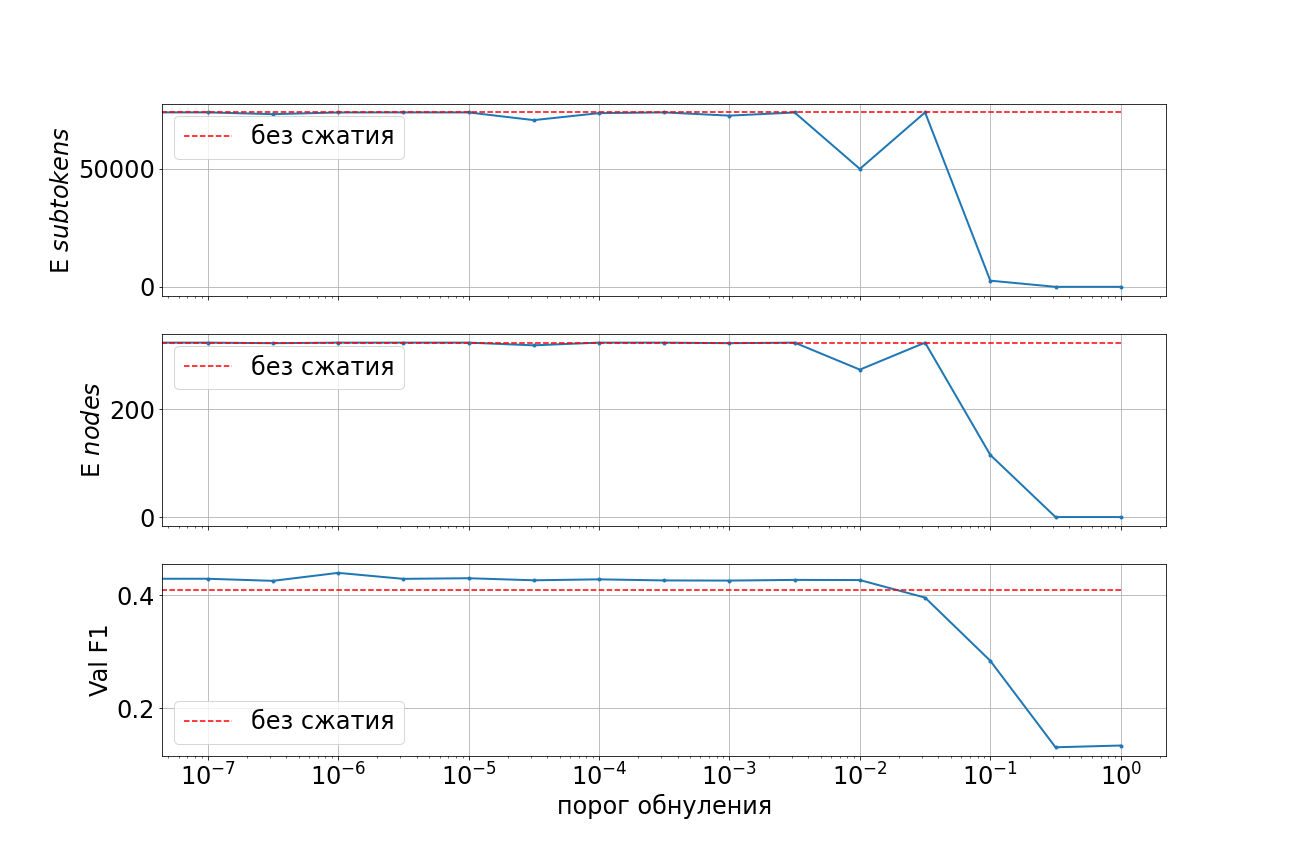
\includegraphics[width=0.8\textwidth]{example.png}
	\caption{Пример графика. Тут должна быть подпись, поясняющая что происходит на рисунке (краткая, но достаточная для понимания основной идеи графика).}
	\label{fig:by_epochs}
\end{figure}

Все рисунки в тексте должны иметь подписи и вы на них должны ссылаться в тексте. Например, на Рисунке~\ref{fig:by_epochs} изображен пример графика. Не забывайте подписывать все оси на графиках, добавлять легенду и пояснять все обозначения, а также используйте адекватного размера шрифты и толщину линий на графиках (все должно быть видно и понятно без многократного увеличения). На рисунке из примера явно не хватает обозначения синей линии в легенде.


\subsection{Таблицы}

Все таблицы в тексте тоже должны иметь подписи и вы на них должны ссылаться в тексте. Например, в Таблице~\ref{table:long_epochs} показаны результаты примерного эксперимента. 


\begin{table}[ht]
	\caption{Пример таблички. Тут должна быть подпись, поясняющая что происходит в таблице (краткая, но по делу).}
	\label{table:long_epochs}
	\footnotesize
	\centering
	\begin{tabular}{lrrrrrrrr}
		\toprule
		& \multicolumn{3}{c}{$\mathsf{Val}$} &
		\multicolumn{3}{c}{$\mathsf{Test}$} \\
		\cmidrule(lr){2-4} \cmidrule(l){5-7} 
		{} &  $\mathsf{Prec}$ &  $\mathsf{Rec}$ &  $\mathsf{F1}$ &  $\mathsf{Prec}$ &  $\mathsf{Rec}$ &  $\mathsf{F1}$  &  $\mathsf{nodes}$ & $\mathsf{subtokens}$\\
		\midrule
		запуск 1    &    0.4894 &   0.3775 &  0.4263 &     0.4824 &    0.3683 &   0.4177 & 10029 & 179\\
		запуск 2    &    0.4887 &   0.3739 &  0.4237 &     0.4891 &    0.3724 &   0.4228 & 10039 & 177\\
		запуск 3    &    0.4820 &   0.3751 &  0.4219 &     0.4838 &    0.3677 &   0.4178 & 10037&	180\\
		\midrule
		\bf{среднее} &    \bf{0.4867} &   \bf{0.3755} &  \bf{0.4239} &    \bf{ 0.4851} &    \bf{0.3695} &   \bf{0.4195} \\
		\bf{дисперсия}  &    0.0041 &   0.0019 &  0.0022 &     0.0036 &    0.0025 &   0.0029 \\
		\bottomrule
	\end{tabular}
\end{table}

\subsection{Формулы}

Формулы стоит центрировать, а также нумеровать, если вы ссылаете на них в тексте. Также не забывайте пояснять все обозначения в формулах. Например, запишем следующую задачу оптимизации:
\begin{equation}
    \label{eq:si_opt}
        \theta* = \min_{\theta} F(\theta),
\end{equation}
где $F$~-- квадратичная функция от параметра $\theta$. При необходимости, далее в тексте можно сослаться на формулу~(\ref{eq:si_opt}). При этом, в зависимости от конкретных формул, можно использовать разные слова: формула, уравнение, задача оптимизации и т.п.


	
\newpage 
\printbibliography[heading=bibintoc] 

% \begin{thebibliography}{0}
% 	\bibitem{chirkova18}\hypertarget{chirkova18}{}
% 	\href{https://arxiv.org/abs/1810.10927}
% 	{Nadezhda Chirkova, Ekaterina Lobacheva, Dmitry Vetrov. Bayesian Compression for Natural Language Processing. In EMNLP 2018.}
% \end{thebibliography}

\newpage
\appendix

\section{Пример секции аппендикса}

\end{document}
